\newpage
\section{Materiais e métodos}

% =============== INTRODUÇÃO ===================== %
\subsection{O fator $\gamma$ do ar}

O coeficiente de expansão adiabática, representado pela letra grega $\gamma$, é a razão entre a capacidade térmica a pressão constante e a capacidade térmica a volume constante de um gás, ou seja:

\[ \gamma = \frac{c_P}{c_V} \]

Nesse tipo de transformação - adiabática -, o sistema não troca calor com o ambiente; o trabalho realizado é referente à variação de energia interna do sistema. Numa expansão adiabática, o sistema realiza trabalho sobre o meio e a energia interna diminui. Na expansão adiabática ocorre um abaixamento de temperatura.\\

Pela Lei dos Gases Ideais, juntamente do Teorema da Equipartição de Energia e, também, por outras equações de termodinâmica, pode-se chegar às equações que relacionam $\gamma$ com as capacidades caloríficas a volume e pressão constantes ($C_V$ e $C_P$, respectivamente).\\

Desse modo, como o calor específico pode ser obtido pela divisão da capacidade calorífica pela massa, conseguimos obter a equação que relaciona $\gamma$ com $c_V$ e $c_P$ - já citada acima -, equação que será base para nossos primeiros experimentos.

% =============== EXPERIMENTOS ===================== %

\subsection{Fator $\gamma$ do ar: Método de Clément – Desormes}

Para esse primeiro experimento, já explicado na seção anterior, buscaremos encontrar o coeficiente $\gamma$ do ar utilizando o método de Clément -  Desormes. O esquema dos passos que seguiremos está logo abaixo:

\begin{figure}[H]
  \centering
  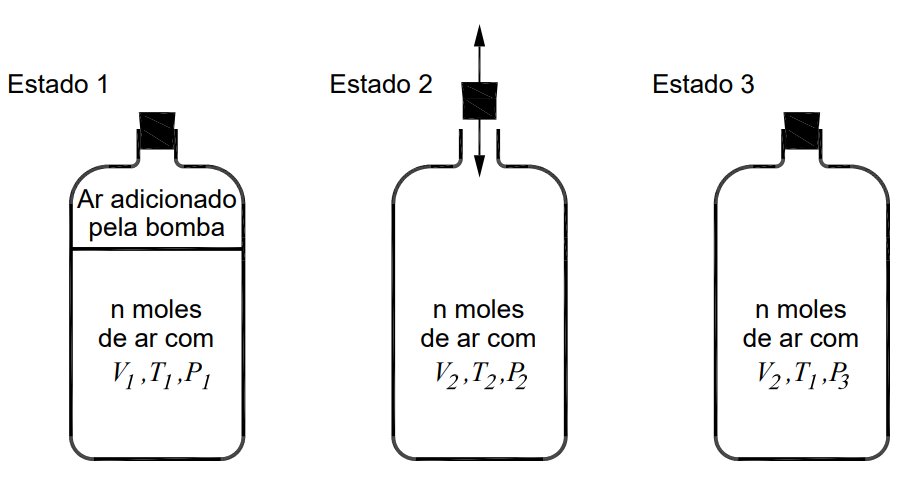
\includegraphics[scale=0.67]{images/Esquema exp.png}
  \caption{Esquema dos três estados que consideramos no processo experimental de Clément-Desormes.}
\end{figure}

Os 3 estados presentes no esquema acima, representam os pontos destacados na Figura \ref{fig:processo-grafico}. Assim, tendo explicitado nosso experimento, podemos dar iniciá-lo.

Primeiramente, vamos tampar a garrafão e bombear manualmente uma certa quantidade de ar para dentro dele, para aumentar a pressão interna. Olhando para o manômetro, esperaremos que o sistema se estabilize - à temperatura ambiente $T_1$ e uma dada pressão $P_1$ (a utilizaremos em função da diferença de altura $h_1$ lida no manômetro).
Chamaremos essa configuração de Estado Inicial ou Estado 1.

Com base na observação do vídeo do experimento, podemos dizer que a altura $h_1$ é a diferença de altura da coluna maior para a menor:\ 
\ \[h_1 = h_{maior} - h_{menor} \]
\[\therefore h_1 = 223,2 cm - 205,2 cm  =  18,0 cm\]
A incerteza de $h_1$ será:\\
\[\delta h_1 = 0,1 cm + 0,1 cm =  0,2 cm\]
\[\therefore h_1 = 18,0 \pm 0,2 cm\]


\begin{figure}[H]
  \centering
  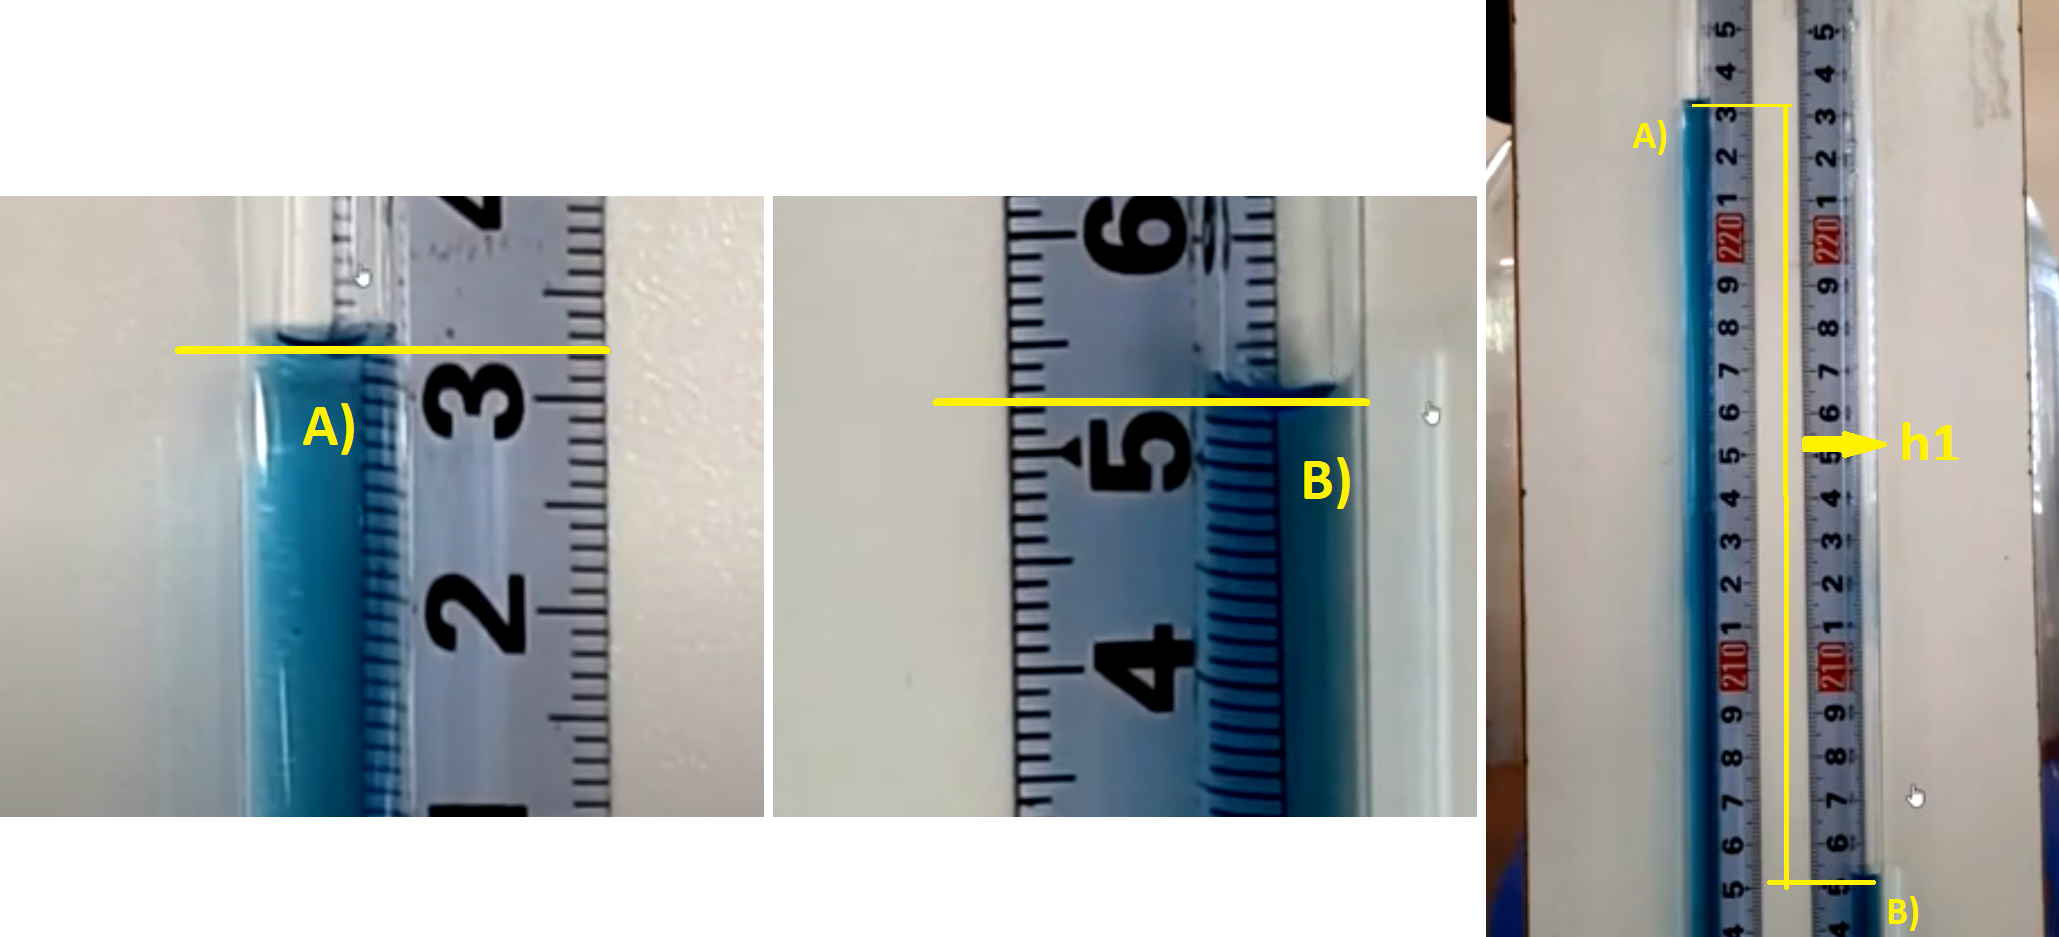
\includegraphics[scale=0.37]{images/Medida 1.1.png}
  \caption{Medida da altura $h_1$ no manômetro (1°experimento).}
\end{figure}

Agora, vamos abrir e fechar a válvula do garrafão. Dessa forma, a pressão interna deve se igualar à pressão atmosférica ($P_2$ = $P_{atm}$). O processo de abrir e fechar o sistema é muito rápido, assim, o gás não tem tempo de trocar calor com o ambiente nesse curto período de tempo, além disso, o vidro do garrafão é um péssimo condutor de calor. Logo, podemos considerar esse processo como adiabático. Ao fechar o tampão da garrafa, chegamos ao Estado Intermediário ou Estado 2, da Figura \ref{fig:processo-grafico}.\\

Logo após a expansão adiabática ocorrer, o gás deve estar em uma temperatura $T_2$ ligeiramente menor que a temperatura ambiente $T_{amb}$ = $T_1$. Após um tempo, a temperatura do sistema irá aumentar e se igualar à temperatura ambiente $T_1$. As paredes rígidas do garrafão garantem que o processo ocorra a volume constante $V_2$ (processo isocórico). Assim que o gás atingir a temperatura $T_1$, estaremos no Estado Final ou Estado 3 pela Figura \ref{fig:processo-grafico}. A pressão nesse ponto ($P_3$) pode ser dada em função da altura $h_3$, que será encontrada a seguir:\

\ \[h_3 = h_{maior} - h_{menor} \]
\[\therefore h_3 = 216,9 cm - 211,3 cm  =  5,6 cm\]
A incerteza de $h_3$ será:\\
\[\delta h_3 = 0,1 cm + 0,1 cm =  0,2 cm\]
\[\therefore h_3 = 5,6 \pm 0,2 cm\]


\begin{figure}[H]
  \centering
  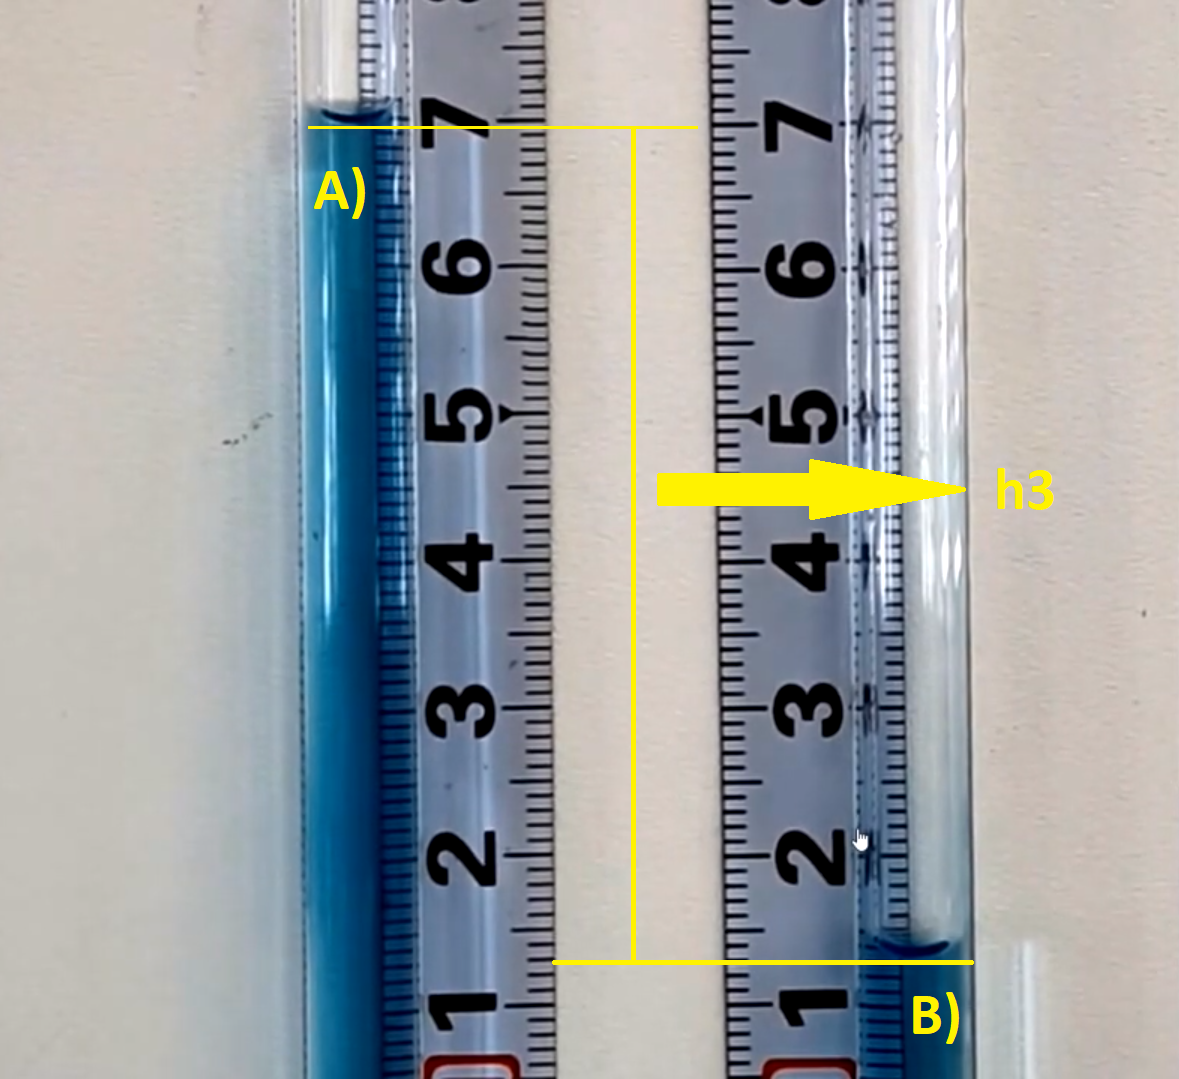
\includegraphics[scale=0.4]{images/Medida 2.1.png}
  \caption{Medida da altura $h_3$ no manômetro (1°experimento).}
\end{figure}

Dessa maneira, conseguimos achar $\gamma$ em função das alturas $h_1$ e $h_3$, como explicitado na seção anterior:\ 

\[ \gamma = \frac{h_1}{h_1 - h_3}\]
\[ \gamma = \frac{18,0}{18,0 - 5,6} = \frac{18,0}{12,4} \]
\[\therefore \gamma = 1,4516129 \approx 1,45\]
E a incerteza de $\gamma$ será:\\
\[\delta \gamma = \frac{(\delta h_1 \cdot h_1 - h_3)+((\delta h_1) + \delta h_3)) \cdot h_1)}{(h_1 - h_3)^2}\]
\[\delta \gamma = \frac{(0,1 \cdot 12,4)+(0,2 \cdot 18,0)}{(12,4)^2}\]
\[\delta \gamma = \frac{4,84}{153,76} = 0,0314776 \approx 0,03\]
Logo:\\ 
\[\therefore \gamma_1 = 1,45 \pm 0,03 \]

Agora, vamos repetir todo esse processo mais duas vezes para poder calcular média e desvio padrão dos nossos valores para o coeficiente $\gamma$, e assim, obter um resultado mais satisfatório.

Na segunda medição, chegamos ao Estado 1 novamente, e medimos nosso $h_1$ - nas mesmas condições que da primeira vez -, que agora ficou:\\

\ \[h_1 = h_{maior} - h_{menor} \]
\[\therefore h_1 = 222,2 cm - 206,1 cm  =  16,1 cm\]
A incerteza de $h_1$ será:\\
\[\delta h_1 = 0,1 cm + 0,1 cm =  0,2 cm\]
\[\therefore h_1 = 16,1 \pm 0,2 cm\]

\begin{figure}[H]
  \centering
  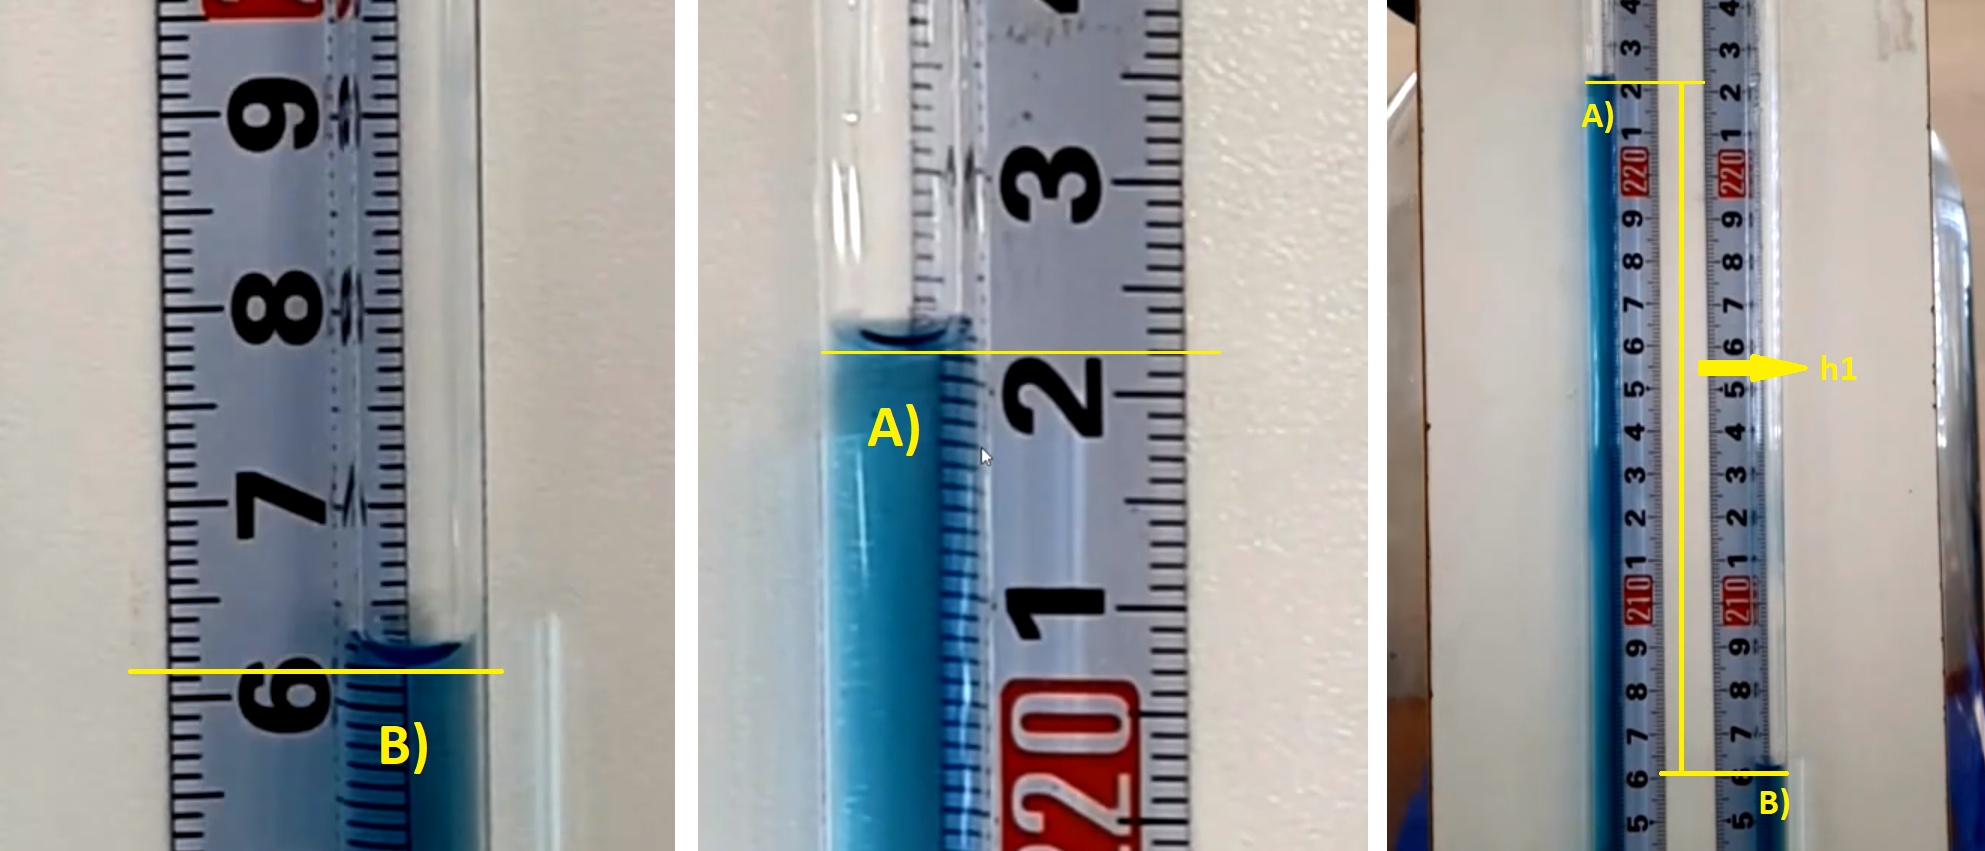
\includegraphics[scale=0.37]{images/Medida 1.2.png}
  \caption{Medida da altura $h_1$ no manômetro (2°experimento).}
\end{figure}

Assim, realizamos o processo adiabático de 1 até 2, e nesse Estado pudemos notar que $T_2$ era menor que $T_1$ e que  $P_2$ = $P_{atm}$, como antes. Depois disso, a temperatura subiu até se igualar à temperatura ambiente $T_1$. Esse processo isocórico, nos leva do Estado 2 para o Estado 3, e a pressão $P_3$ pode ser dada em relação à medida $h_3$ averiguada no manômetro:

\ \[h_3 = h_{maior} - h_{menor} \]
\[\therefore h_3 = 216,1 cm - 212,1 cm  =  4,0 cm\]
A incerteza de $h_3$ será:\\
\[\delta h_3 = 0,1 cm + 0,1 cm =  0,2 cm\]
\[\therefore h_3 = 4,0 \pm 0,2 cm\]


\begin{figure}[H]
  \centering
  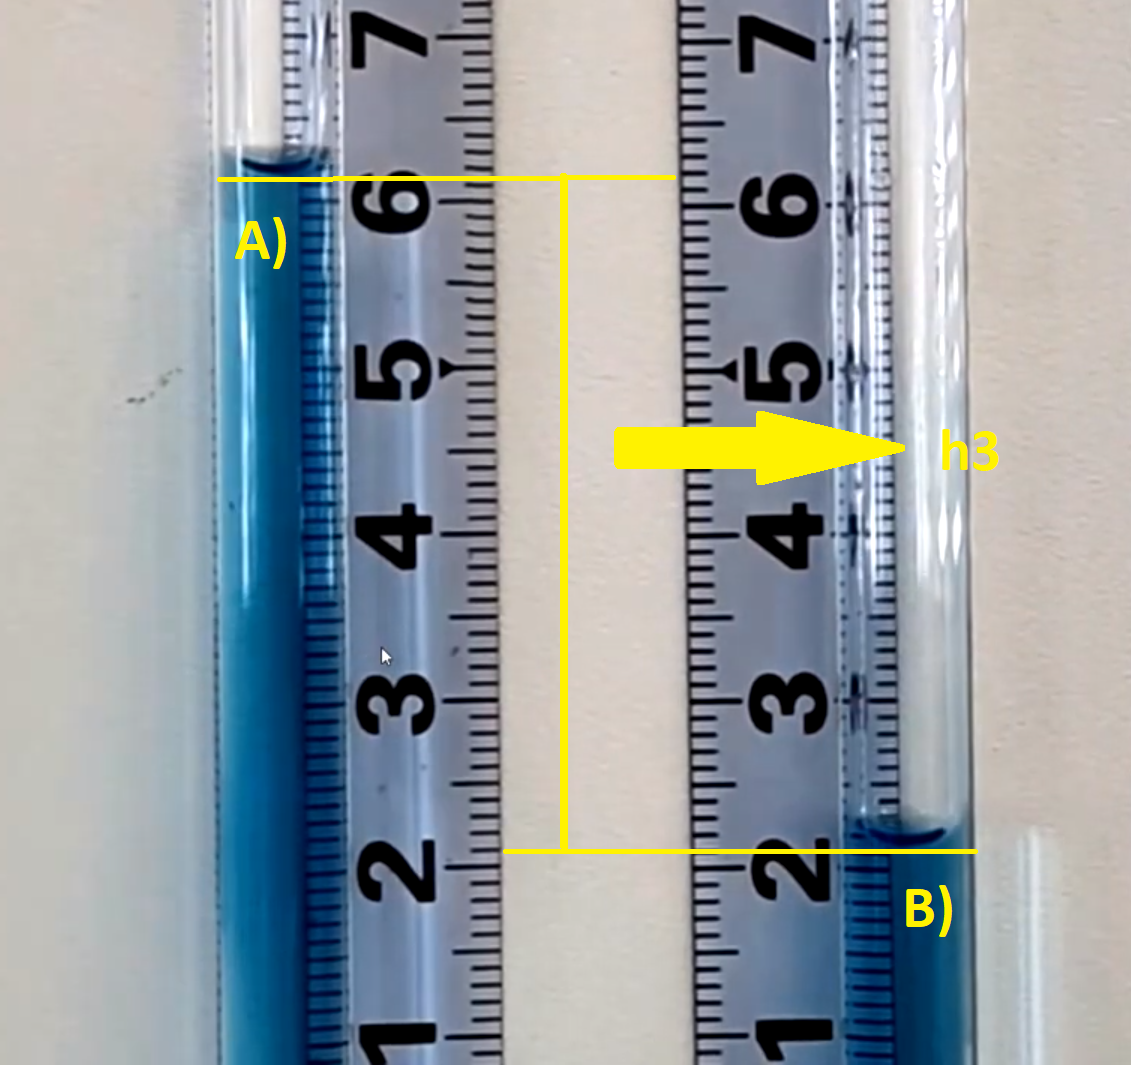
\includegraphics[scale=0.4]{images/Medida 2.2.png}
  \caption{Medida da altura $h_3$ no manômetro (2°experimento).}
\end{figure}

Logo, podemos achar $\gamma$ em função das alturas $h_1$ e $h_3$:\\

\[ \gamma = \frac{h_1}{h_1 - h_3}\]
\[ \gamma = \frac{16,1}{16,1 - 4,0} = \frac{16,1}{12,1} \]
\[\therefore \gamma = 1,3305785 \approx 1,33\]
E a incerteza de $\gamma$ será:\\
\[\delta \gamma = \frac{(\delta h_1 \cdot h_1 - h_3)+((\delta h_1) + \delta h_3)) \cdot h_1)}{(h_1 - h_3)^2}\]
\[\delta \gamma = \frac{(0,1 \cdot 12,1)+(0,2 \cdot 16,1)}{(12,1)^2}\]
\[\delta \gamma = \frac{4,43}{146,41} = 0,0302575 \approx 0,03\]
Logo:\\ 
\[\therefore \gamma_2 = 1,33 \pm 0,03 \]

Por último, faremos as mesmas medidas pela terceira vez, buscando $h_1$ e $h_3$ para o cálculo de $\gamma$, então, vamos apresentar diretamente os valores das alturas, uma vez que o processo já foi explicado acima, e vamos realizá-lo identicamente.\\

No Estado 1, teremos:\\

\ \[h_1 = h_{maior} - h_{menor} \]
\[\therefore h_1 = 223,0 cm - 205,3 cm  =  17,7 cm\]
A incerteza de $h_1$ será:\\
\[\delta h_1 = 0,1 cm + 0,1 cm =  0,2 cm\]
\[\therefore h_1 = 17,7 \pm 0,2 cm\]

\begin{figure}[H]
  \centering
  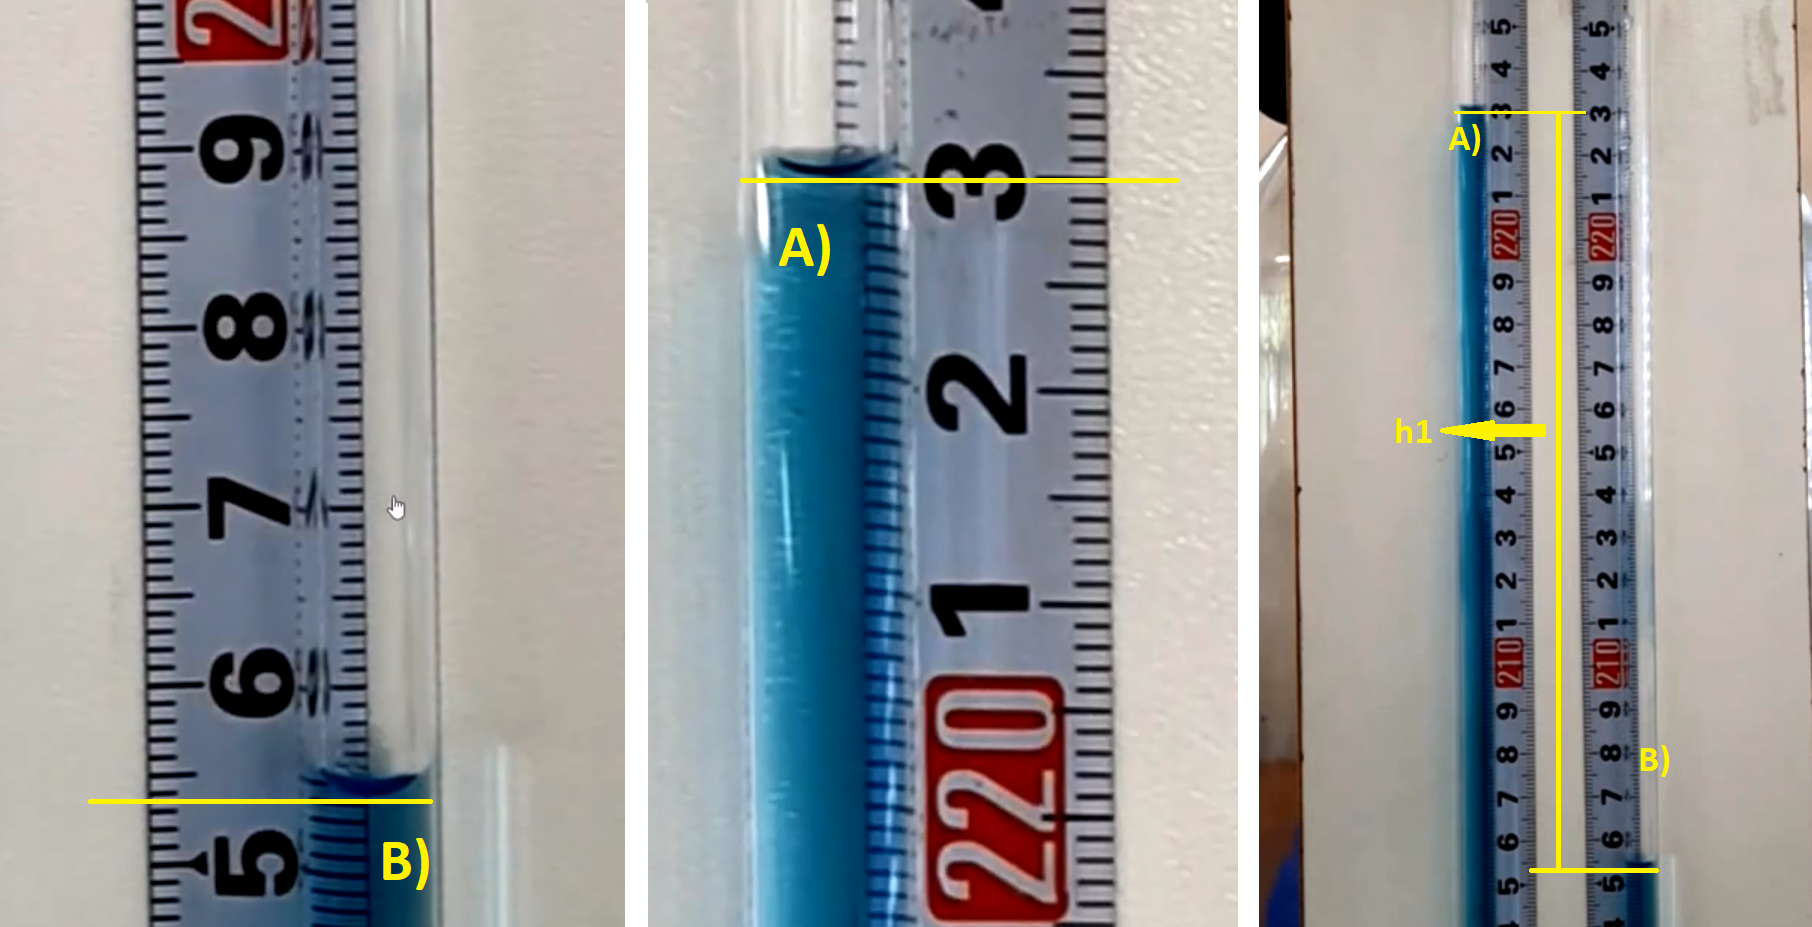
\includegraphics[scale=0.37]{images/Medida 1.3.png}
  \caption{Medida da altura $h_1$ no manômetro (3°experimento).}
\end{figure}

Já para o Estado 3:\\

\ \[h_3 = h_{maior} - h_{menor} \]
\[\therefore h_3 = 216,7 cm - 211,6 cm  = 5,1 cm\]
A incerteza de $h_3$ será:\\
\[\delta h_3 = 0,1 cm + 0,1 cm =  0,2 cm\]
\[\therefore h_3 = 5,1 \pm 0,2 cm\]


\begin{figure}[H]
  \centering
  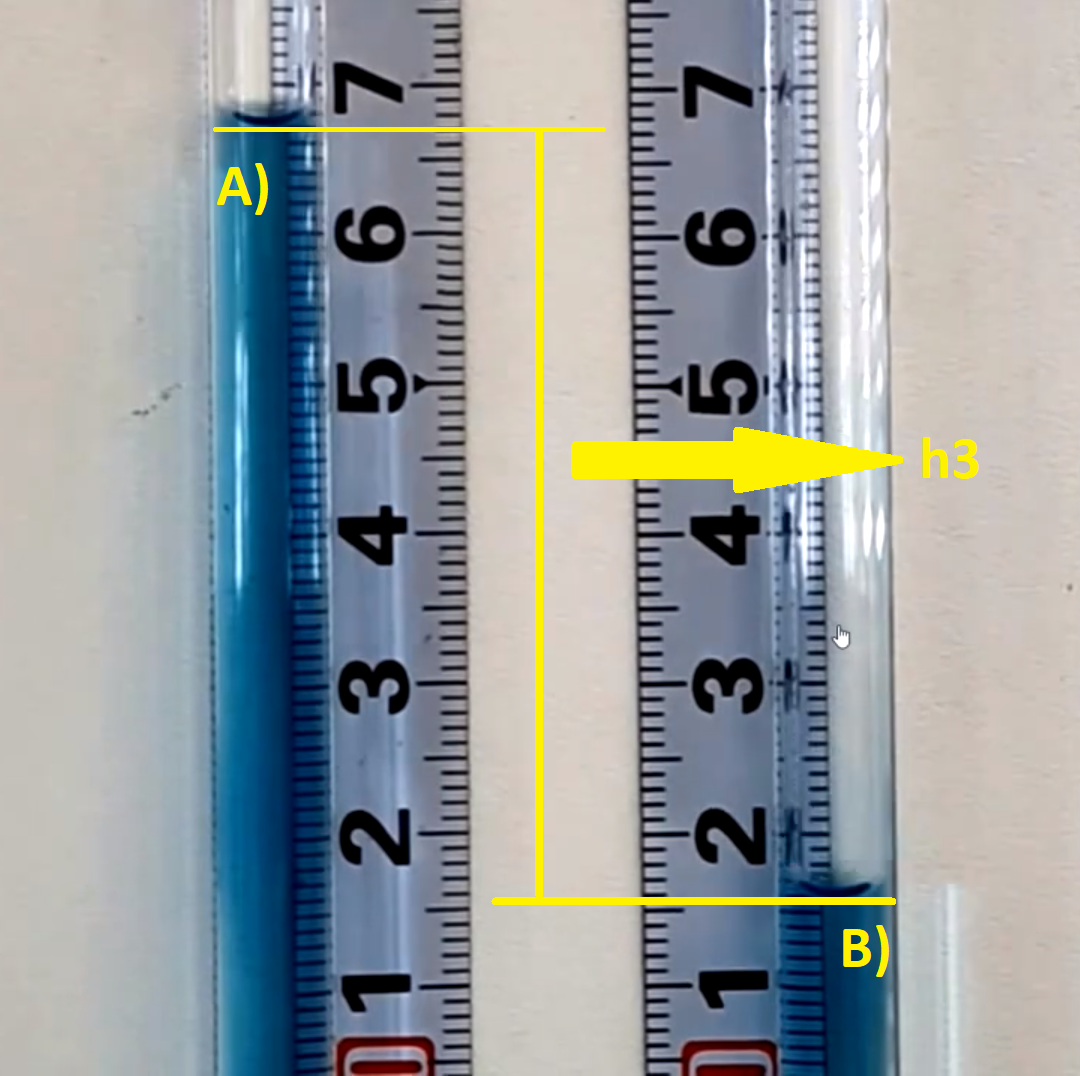
\includegraphics[scale=0.4]{images/Medida 2.3.png}
  \caption{Medida da altura $h_3$ no manômetro (3°experimento).}
\end{figure}

Com as alturas $h_1$ e $h_3$ calculadas, conseguimos obter o coeficiente $\gamma$:\\

\[ \gamma = \frac{h_1}{h_1 - h_3}\]
\[ \gamma = \frac{17,7}{17,7 - 5,1} = \frac{17,7}{12,6} \]
\[\therefore \gamma = 1,4047619 \approx 1,40 \]
E a incerteza de $\gamma$ será:\\
\[\delta \gamma = \frac{(\delta h_1 \cdot h_1 - h_3)+((\delta h_1) + \delta h_3)) \cdot h_1)}{(h_1 - h_3)^2}\]
\[\delta \gamma = \frac{(0,1 \cdot 12,6)+(0,2 \cdot 16,1)}{(12,6)^2}\]
\[\delta \gamma = \frac{4,48}{158,76} = 0,02821869 \approx 0,03\]
Logo:\\ 
\[\therefore \gamma_3 = 1,40 \pm 0,03 \]

Assim, até agora obtivemos os seguintes valores para $\gamma$ nos 3 experimentos analisados:\\
\[\gamma_1 = 1,45 \pm 0,03\]
\[\gamma_2 = 1,33 \pm 0,03\]
\[\gamma_3 = 1,40 \pm 0,03\]

Tendo esses valores, podemos então calcular a média e o desvio padrão desses resultados.\\
\subsection{Fator $\gamma$ do ar: Método de Rüchardt}

Como introduzido no experimento anterior, o fator $\gamma$ é uma propriedade intrínseca dos gases, muito interessante e importante se ter conhecimento. Para isso, utilizaremos agora uma outra forma de determiná-lo.

Nesse experimento, elaborado pelo físico alemão Eduard Rüchardt, utilizaremos o mesmo princípio do anterior: pressurizaremos um recipiente com uma bomba manual e liberaremos rapidamente esse ar para realizar aquele processo termodinâmico como visto na Figura \ref{fig:processo-grafico}.

A diferença aqui virá do fato que temos na montagem experimental uma bolinha que se encontra em equilíbrio com a pressão interna e a atmosférica, pois ela cria uma vedação com o tudo alongado. Isso quer dizer que qualquer variação de pressão dentro do recipiente (provocada por um processo de compressão e rápida descompressão, por exemplo) ocasionará um movimento nela.

\begin{figure}[H]
  \centering
  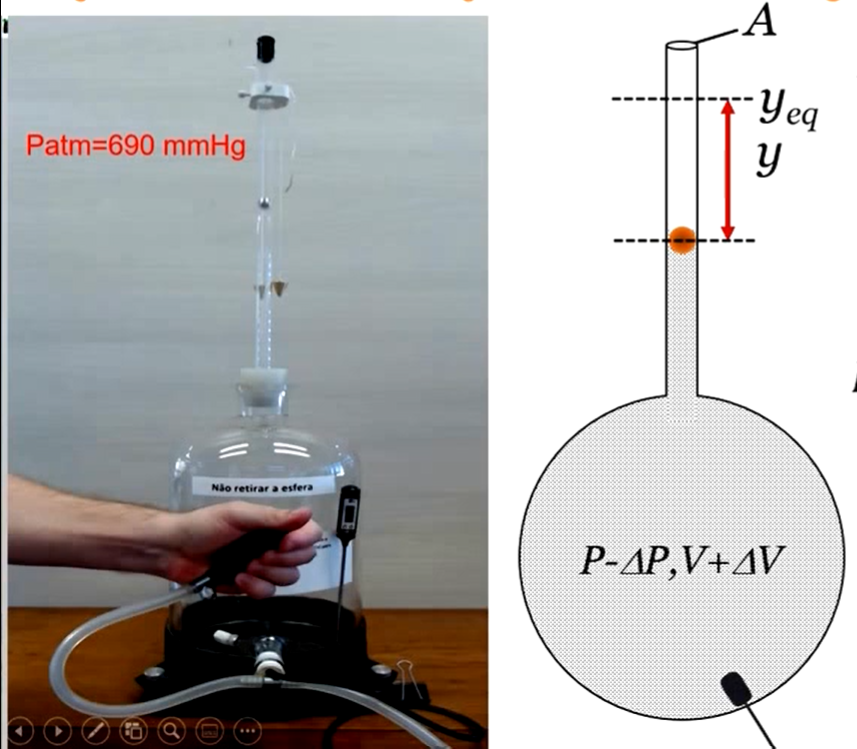
\includegraphics[scale=0.7]{images/montagem-ruchardt.png}
  \caption{Montagem experimental e diagrama do Método de Rüchardt}
\end{figure}

Desenvolvendo as equações de equilíbrio de forças presentes nesse experimento que foram vistas na videoaula dessa prática, chegamos na seguinte relação:

\[ \ddot{y} + \left( \frac{\gamma P A^2}{m V} \right) y = 0 \]

Essa equação é característica de um movimento harmônico, ou seja, a bolinha oscilará (amortecidamente, já que vivemos num mundo não ideal onde existe atrito e resistência do ar) no final do processo. Sendo assim, medindo o período de oscilação (T) nós podemos encontrar o desejado $\gamma$ do ar atmosférico.\\

Então, utilizaremos um microfone interno para captar as variações periódicas de pressão, e com um software de análise sonora podemos obter o período mencionado. Com esse valor e as características dos equipamentos e ambiente em mãos, como a massa da boinha (m), área do tubo (A), volume do recipiente (V) e a pressão atmosférica (P), podemos falar que a característica $\gamma$ do ar pode ser definida como:

\[ N = m \cdot V \]
\[ D = P \cdot A^2 \cdot T^2 \]
\[ \therefore \gamma = 4\pi^2 \cdot \frac{N}{D} \]

E a sua incerteza \textbf{VERIFICAR ISSO AQUI PQ PODE N ESTAR CERTO}:

\begin{table}[H]
    \centering
    \begin{tabular}{ c|c  }
         $\delta N = \delta m \cdot V + m \cdot \delta V$ &
         $\delta a = 2 \cdot A \cdot \delta A$\\
         \hline \\
         $\delta D = P \cdot (A \cdot \delta t + \delta a \cdot T)$ &
         $\delta t = 2 \cdot T \cdot \delta T$\\
    \end{tabular}
\end{table}

\[ \therefore \delta \gamma = 4\pi^2 \cdot \frac{N \cdot \delta D + \delta N \cdot D}{D^2}\]

*as fórmulas foram quebradas para facilitar nos cálculos

\subsection{Zero absoluto: Determinação do zero absoluto utilizando um termômetro a
gás}

Conforme a descrição na metodologia, os primeiros dados coletados neste experimento foram os relativos às pressões do gás do sistema para determinadas temperaturas descritas nas quatro condições a seguir:

\begin{enumerate}
    \item Bulbo mergulhado em água à temperatura ambiente;
    \item Bulbo mergulhado em gelo em fusão;
    \item Bulbo mergulhado em nitrogênio líquido;
    \item Bulbo mergulhado em água em ebulição.
\end{enumerate}

Lembrando que as pressões são determinadas diretamente pela leitura da altura h da coluna no experimento, sendo que h é obtido pela diferença das alturas em dois pontos distintos do termômetro em “U”. Dessa forma, temos a seguinte tabela com os dados, numerados de acordo com cada condição:

\begin{table}[H]
    \centering
    \begin{tabular}{ |c||c||c| }
        \hline
        \textbf{Condição} & \textbf{Temperatura (ºC)} & \textbf{Pressão (cmHg)}\\
        \hline 
        1       & 24,7     & $h = 81 - 12 = 69$  \\
        2       & 1,0      & $h = 78 - 15 = 63$  \\
        3       & -196,0   & $h = 55,4 - 37,5 = 17,9$ \\
        4       & 97,0     & $h = 87,8 - 5,5 = 82,3$ \\
        \hline
        \end{tabular}
    \caption{Valores de Temperatura e Pressão para cada condição estabelecida no experimento conforme a enumeração.} 
\end{table}

Após isso, construímos um gráfico da pressão (medida em cmHg) em função da temperatura (medida em ºC), que pode ser visualizado na imagem abaixo:

\begin{figure}[H]
  \centering
  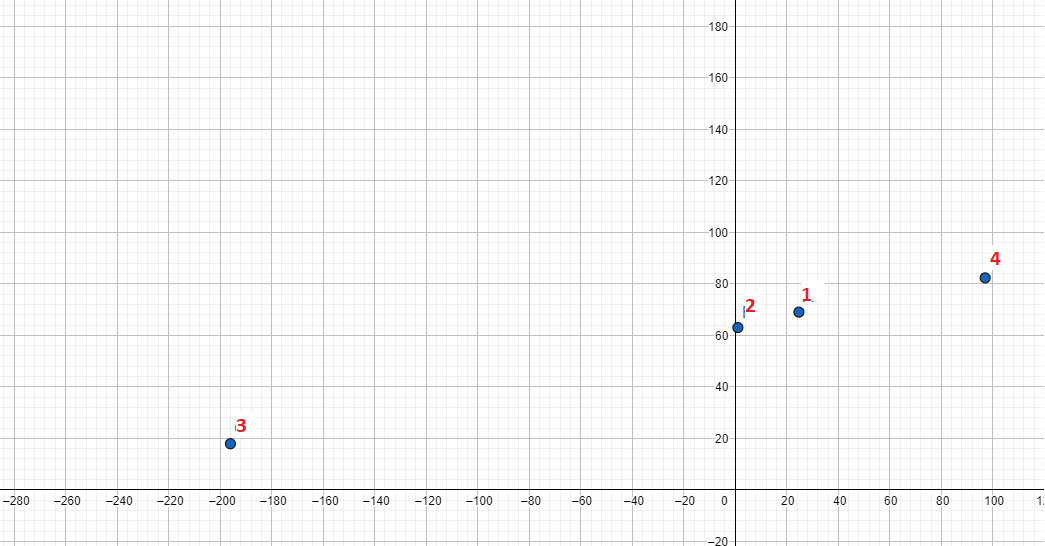
\includegraphics[scale=0.5]{images/Gráfico 1 - experimento 3.png}
  \caption{Gráfico da Pressão (cmHg) em função da Temperatura (ºC).}
\end{figure}

Utilizando o aplicativo “Least Squares” para Android, determinamos o coeficiente de dilatação do gases ideais a volume constante ($\beta$) e o valor de $P_0$ a partir do método dos mínimos quadrados. O resultado da aplicação desse método pode ser visualizado na imagem a seguir:

\begin{figure}[H]
  \centering
  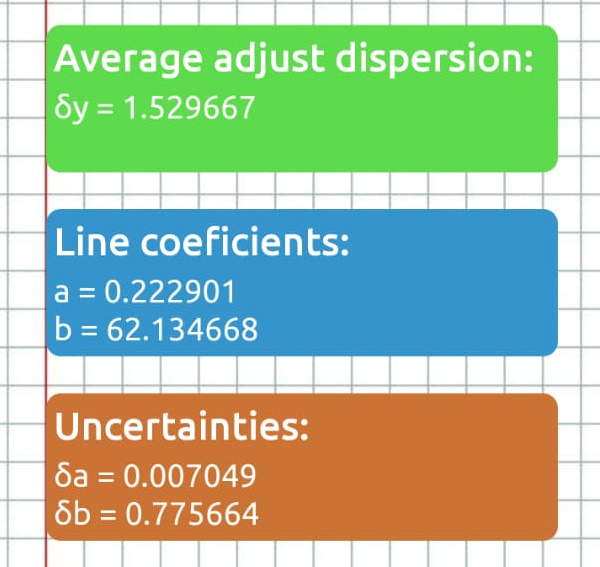
\includegraphics[scale=0.6]{images/Gráfico 2 - experimento 3.png}
  \caption{Aplicação do Método dos Mínimos Quadrados para encontrar os valores do coeficiente angular (a) e do coeficiente linear (b).}
\end{figure}

Na análise gráfica, determinamos, então, o coeficiente de dilatação dos gases ideais a volume constante $\beta$ e o valor de $P_0$:

\[ b (\textbf{coeficiente linear}) = P_0 = (62,1 \pm 0,8) cmHg\]\
\[ a (\textbf{coeficiente angular}) = P_0 \cdot \beta \longrightarrow \beta = \frac{(0,223 \pm 0,007)}{(62,1 \pm 0,8)} = (0,0036 \pm 0,0002) \]\

Portanto, sabendo os valores de $\beta$ e $P_0$, podemos escrever a equação que descreve esse comportamento do gráfico da pressão (medida em cmHg) em função da temperatura (medida em ºC), sendo igual a:

\[ P(T) = P_0 \cdot \beta \cdot T + P_0 \]\
\[ P(T) = (62,1 \pm 0,8) \cdot (0,0036 \pm 0,0002) \cdot T + (62,1 \pm 0,8) \]\
\[ \therefore P(T) = (0,223 \pm 0,007) \cdot T + (62,1 \pm 0,8) \]\

Após a determinação da equação acima, traçamos uma reta sobre os pontos experimentais e determinamos, com a extrapolação dessa reta, o zero absoluto:

\begin{figure}[H]
  \centering
  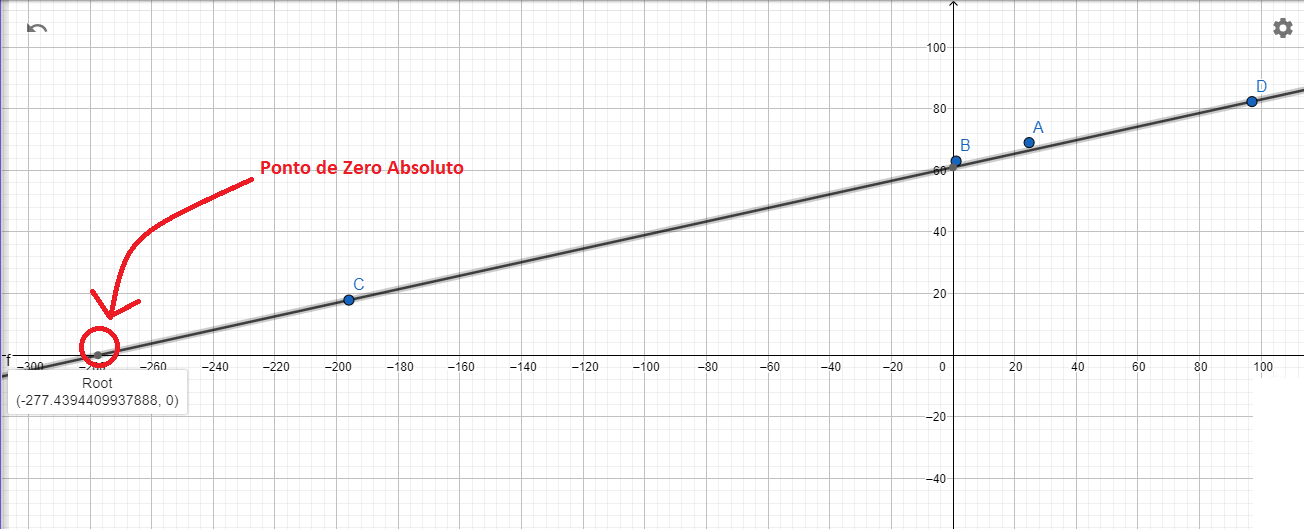
\includegraphics[scale=0.45]{images/Gráfico 3 - experimento 3.png}
  \caption{Equação da reta que define a pressão do gás em função da temperatura com sua respectiva extrapolação para determinação do zero absoluto.}
\end{figure}

Dessa forma, após uma análise gráfica, podemos determinar o valor correspondente do ponto de zero absoluto a partir de cálculos diretamente da equação que define a reta, lembrando que no zero absoluto a pressão do gás é dita conceitualmente igual a 0: 

\[ P(T) = P_0 \cdot \beta \cdot T + P_0 \]\
\[ 0 = (0,223 \pm 0,007) \cdot T + (62,1 \pm 0,8) \]\
\[ -(62,1 \pm 0,8) = (0,223 \pm 0,007) \cdot T  \]\
\[ \frac{-(62,1 \pm 0,8)}{(0,223 \pm 0,007)}  =  T  \]\
\[ \therefore \mathbf{T = -(278 \pm 5) ^\circ C} \]\

Dessa forma, podemos concluir que o valor correspondente do ponto de zero absoluto é igual a $T_{Zero-Absoluto}= -(278 \pm 5) ^\circ C$. Conforme a literatura científica, a temperatura de zero absoluto é de aproximadamente $T_{Zero-Absoluto-Ref}= -273 ^\circ C$, ou seja, podemos concluir que o valor alcançado experimentalmente é \textbf{satisfatório} dado que é equivalente ao valor de referência se considerarmos a sua respectiva incerteza.

